\documentclass[xcolor=svgnames,9pt,english,aspectratio=169,t]{beamer}
%\documentclass[xcolor=svgnames,9pt,english,handout,aspectratio=169,t]{beamer}
\newcommand{\handout}{0}
% Public release: the repository copy sets \releasetrue, which drops this term's logistics
% (times, dates, rooms, staff, Canvas). Leave it false for the course build.
\newif\ifrelease
\releasetrue

% =====================================================================
% POLI 450A (2026) --- shared TEMPLATE layer.
%
% Input from each lecture near the top of its file, BEFORE
% ../course_theme.tex (metropolis must be selected before the course
% palette overrides it):
%
%   \documentclass[xcolor=svgnames,9pt,english,aspectratio=169]{beamer}
%   \newcommand{\handout}{0}
%   % =====================================================================
% POLI 450A (2026) --- shared TEMPLATE layer.
%
% Input from each lecture near the top of its file, BEFORE
% ../course_theme.tex (metropolis must be selected before the course
% palette overrides it):
%
%   \documentclass[xcolor=svgnames,9pt,english,aspectratio=169]{beamer}
%   \newcommand{\handout}{0}
%   % =====================================================================
% POLI 450A (2026) --- shared TEMPLATE layer.
%
% Input from each lecture near the top of its file, BEFORE
% ../course_theme.tex (metropolis must be selected before the course
% palette overrides it):
%
%   \documentclass[xcolor=svgnames,9pt,english,aspectratio=169]{beamer}
%   \newcommand{\handout}{0}
%   \input{../course_preamble.tex}
%   \input{../course_theme.tex}
%   \graphicspath{{./}{./figs/}}
%   \title[Short title]{450A Political Methodology I}
%   \subtitle{Lecture N: ...}
%
% Modeled on the 2026 Northwestern workshop template
% (Teaching/PanelData/_latex/2026/202608_Northwestern/workshop_preamble.tex).
%
% SCOPE: theme, beamer layout, packages, the roadmap hooks, and --- unlike
% the Northwestern decks --- the notation macros. The 450A lectures
% grew from one common ancestor, so their macro blocks agree wherever they
% overlap; merging them is safe. Three points where they had drifted are
% resolved here, and each is flagged inline below.
% =====================================================================

\usetheme{metropolis}
\metroset{sectionpage=none, subsectionpage=none, numbering=none}
\setbeamertemplate{navigation symbols}{}

\setbeamersize{text margin left=5mm, text margin right=5mm}
\setbeamertemplate{itemize/enumerate body begin}{\leftmargini=1.5em\relax}
\setbeamertemplate{itemize/enumerate subbody begin}{\leftmarginii=1.5em\relax}
\setbeamertemplate{itemize/enumerate subsubbody begin}{\leftmarginiii=1.5em\relax}

% ----------------------------------------------------------- top alignment
% Every deck passes the t class option, so beamer applies the frame key
% below to every frame (explicit [plain,c] frames — title page, roadmaps —
% stay centered). Beamer's stock t key puts a rigid .2cm pad above the
% content; frames sized to this template's full-height ceilings then run
% Overfull \vbox by up to that pad. Same key as beamerbaseframe.sty, with
% one change: the pad may shrink to zero when the frame is full.
\makeatletter
\define@key{beamerframe}{t}[true]{% top
  \beamer@frametopskip=.2cm plus .5\paperheight minus .2cm\relax%
  \beamer@framebottomskip=0pt plus 1fill\relax%
  \beamer@frametopskipautobreak=\beamer@frametopskip\relax%
  \beamer@framebottomskipautobreak=\beamer@framebottomskip\relax%
}

% ------------------------------------------------- slide-top check (2026-10-11)
% A slide whose content is too tall for the frame is squeezed: the pad above
% shrinks and its content starts higher than on other slides, so a figure
% "wobbles" when the class steps from one slide to the next (Lecture 4-1,
% slides 1-2, 2026-10-11). The marker below records where each slide's
% content starts (a whatsit: it adds no space and moves nothing).
% `python3 ../check_slides.py lec<N>` then lists every slide that starts
% higher than the deck's normal position. That list must be empty.
% Recorded per slide: page, frame number, content-top y (sp), the room left
% below the title bar, and P for a plain frame (title page, roadmaps).
\providecommand\slidetop[5]{}
\AtBeginDocument{\immediate\write\@auxout{\string\providecommand\string\slidetop[5]{}}}
\def\beamer@markframetop{%
  \pdfsavepos
  \edef\beamer@marktmp{\noexpand\write\noexpand\@auxout{\string\slidetop
    {\noexpand\thepage}{\noexpand\insertframenumber}{\noexpand\the\noexpand\pdflastypos}%
    {\number\beamer@frametextheight}{\ifbeamer@plainframe P\else N\fi}}}%
  \beamer@marktmp}
\RequirePackage{etoolbox}
\patchcmd{\endbeamer@frameslide}
  {\vskip\beamer@frametopskip}
  {\vskip\beamer@frametopskip\beamer@markframetop}
  {}{\PackageWarning{course_preamble}{slide-top marker not installed}}
\makeatother

% ---------------------------------------------------------------- packages
\usepackage{xcolor}
\usepackage{colortbl}
\usepackage{amsmath}
\usepackage{amsfonts}
\usepackage{amssymb}
\usepackage{bm}
\usepackage{graphicx}
\usepackage{multirow}
\usepackage{fancyvrb}
\usepackage{listings}
\usepackage{tikz}
\usetikzlibrary{arrows.meta,positioning,decorations.pathreplacing}

% --------------------------------------------------------- figure fitting
% Default bounding box for every \includegraphics that does not override it.
% With keepaspectratio the image is scaled to fit *inside* width x height, so
% a figure can never run past the side margins or off the bottom of a slide.
% Options given at the call site override these on a per-key basis: e.g.
% [width=.6\linewidth] narrows the box but keeps the height ceiling.
% \figmaxheight is set at \begin{document}: beamer only computes the final
% \textheight once the head/foot templates are known. 0.80 is just under what a
% frame with a title and one line of text can hold (measured: 0.834\textheight);
% a frame that needs more room for text can lower it locally.
\newlength{\figmaxheight}
\AtBeginDocument{\setlength{\figmaxheight}{0.80\textheight}}
\setkeys{Gin}{width=\linewidth,height=\figmaxheight,keepaspectratio}

% -------------------------------------------------------- roadmap frames
% Identical in all lectures. A lecture that does not want the
% subsection roadmap clears it after the \input with \AtBeginSubsection[]{}.
% hideothersubsections is load-bearing, not cosmetic: lecture 4 had 13
% subsections before it was split into 4-1, 4-2 and 4-3 (2026-10-09), and a
% full contents list ran off the top and bottom of the slide. Hiding the other sections' subsections caps the list at 10 lines.
\subject{Talks}
% No back-to-back roadmaps (Yiqing, 2026-10-11): when a subsection starts right
% after its section's roadmap, with no content slide in between, its own
% roadmap would repeat the one just shown (5-1's handout showed "Two Cases"
% twice), so it is skipped. The section roadmap records the frame count; the
% subsection roadmap appears only if a content slide has come since.
\makeatletter
\def\course@secframe{-1}
\AtBeginSection[]
{
  \begin{frame}[plain,c]
    \frametitle{}
    \tableofcontents[currentsection,hideothersubsections]
    \addtocounter{framenumber}{-1}
  \end{frame}
  \xdef\course@secframe{\the\c@framenumber}
}
\AtBeginSubsection[]
{
  \ifnum\c@framenumber=\course@secframe\relax\else
  \begin{frame}[plain,c]
    \frametitle{}
    \tableofcontents[currentsection,currentsubsection,hideothersubsections]
    \addtocounter{framenumber}{-1}
  \end{frame}
  \fi
}
\makeatother

% ------------------------------------------------------ theorem environments
\newtheorem{assumption}{Assumption}
\newtheorem{iass}{Identification Assumption}
\newtheorem{ires}{Identification Result}
\newtheorem{estm}{Estimand}
\newtheorem{esti}{Estimator}
\newtheorem{question}{Question}
\newtheorem{answer}{Answer}
\newtheorem{proposition}{Proposition}

% =====================================================================
% Notation
% =====================================================================
\definecolor{dgreen}{rgb}{0,.6,0.8}

\renewcommand\r{\right}
\renewcommand\l{\left}
\newcommand{\bs}{\boldsymbol}
\newcommand{\mb}{\mathbf}
\newcommand{\real}{\mathbb{R}}
\newcommand{\cN}{\mathcal{N}}
\newcommand{\E}{\mathbb{E}}
\newcommand{\V}{\mathbb{V}}

% MERGE NOTE 1. Lecture 2-4 set \epsilon to \varepsilon; the other twelve
% left it at the upright default. Adopting \varepsilon course-wide so the
% error term looks the same in every lecture.
\renewcommand{\epsilon}{\varepsilon}

% MERGE NOTE 2. Lecture 2-4 wrote its vectors as \bm (bold italic); the other
% twelve use \mathbf (bold upright). \mathbf wins --- it is the convention in
% eleven of the thirteen decks and in the course's matrix lectures. Only
% \iid, \E, \cN and \Var from that block are actually used in 2-4's body.
\renewcommand{\u}{\ensuremath{\mb{u}}}
\renewcommand{\v}{\ensuremath{\mb{v}}}
\newcommand{\U}{\ensuremath{\mb{U}}}
\newcommand{\M}{\ensuremath{\mb{M}}}
\newcommand{\X}{\ensuremath{\mb{X}}}
\newcommand{\x}{\ensuremath{\mb{x}}}
\newcommand{\y}{\ensuremath{\mb{y}}}
\newcommand{\Z}{\ensuremath{\mb{Z}}}
\newcommand{\C}{\ensuremath{\mb{C}}}
\newcommand{\D}{\ensuremath{\mb{D}}}
\newcommand{\I}{\ensuremath{\mb{I}}}
\newcommand{\W}{\ensuremath{\mb{W}}}
\renewcommand{\a}{\ensuremath{\mb{a}}}
\renewcommand{\P}{\ensuremath{\mb{P}}}
\newcommand{\one}{\ensuremath{\mb{1}}}
\newcommand{\zero}{\ensuremath{\mb{0}}}

\renewcommand{\b}{\ensuremath{\bs{\beta}}}
\newcommand{\be}{\ensuremath{\bs{\beta}}}
\newcommand{\e}{\ensuremath{\bs{\epsilon}}}
\newcommand{\eps}{\ensuremath{\bs{\epsilon}}}
\newcommand{\eeta}{\ensuremath{\bs{\eta}}}
\newcommand{\bhat}{\ensuremath{\hat{\bs{\beta}}}}
\newcommand{\ehat}{\ensuremath{\hat{\e}}}
\newcommand{\Sig}{\ensuremath{\bs{\Sigma}}}
\newcommand{\SigInv}{\ensuremath{\bs{\Sigma^{-1}}}}

\newcommand{\XX}{\ensuremath{\X'\X}}
\newcommand{\XXinv}{\ensuremath{\left(\XX\right)^{-1}}}
\newcommand{\hatmat}{\ensuremath{\X \XXinv \X'}}
\newcommand{\hatsig}{\ensuremath{\hat{\sigma}^2}}
\newcommand{\sig}{\ensuremath{\sigma^2}}

\newcommand{\cA}{\mathcal{A}}
\newcommand{\cJ}{\mathcal{J}}
\newcommand{\cL}{\mathcal{L}}
\newcommand{\cLL}{\mathcal{LL}}
\newcommand{\cll}{\ell}
\newcommand{\cQ}{\mathcal{Q}}
\newcommand{\cP}{\mathcal{P}}

% MERGE NOTE 3. \var / \Var and \cov / \Cov were spelled with \text in some
% lectures and \mbox in others. Same output; \text kept.
\newcommand{\var}{\text{Var}}
\newcommand{\Var}{\text{Var}}
\newcommand{\cov}{\text{Cov}}
\newcommand{\Cov}{\text{Cov}}
\newcommand{\cor}{\text{Cor}}
\newcommand{\tr}{\text{tr}}
\newcommand{\avepop}{\frac{1}{n}\sum_{i=1}^n}

\DeclareMathOperator*\plim{plim}
\DeclareMathOperator\rank{rank}
\DeclareMathOperator*\argmax{argmax}
\DeclareMathOperator*\argmin{argmin}
\DeclareMathOperator{\sgn}{sgn}
\newcommand{\diag}{\mathop{\mathrm{diag}}}

\newcommand\ud{\mathrm{d}}
\newcommand\dist{\buildrel\rm d\over\sim}
\newcommand\ind{\stackrel{\rm indep.}{\sim}}
\newcommand\iid{\stackrel{\rm i.i.d.}{\sim}}
\newcommand\logit{{\rm logit}}

\newcommand\indep{\protect\mathpalette{\protect\independenT}{\perp}}
\def\independenT#1#2{\mathrel{\rlap{$#1#2$}\mkern2mu{#1#2}}}

% ------------------------------------------------------------- text helpers
\newcommand{\bi}{\begin{itemize}}
\newcommand{\ei}{\end{itemize}}
\newcommand{\noi}{\noindent}
\newcommand{\red}{\textcolor{Cardinal}}
\newcommand{\blue}{\textcolor{CourseBlue}}
\newcommand{\gray}{\textcolor{gray}}
\newcommand\spacingset[1]{\renewcommand{\baselinestretch}{#1}\small\normalsize}

\hyphenation{tyamamot}


% ------------------------------------------------ figure-position check (2026-10-11)
% Records where every \includegraphics lands and its size (a whatsit; it moves
% nothing). check_slides.py flags two consecutive slides that show a figure of
% the same size in different places: the class sees it jump (Lecture 3, slides
% 18 to 19: one frame had \vspace{.3cm} above the figure, the next did not),
% and two consecutive slides that show the same file at different sizes or
% places (Lecture 6-3, slides 10 to 11, the ballot image). The file name is the
% seventh field.
\makeatletter
\providecommand\figpos[7]{}
\AtBeginDocument{\immediate\write\@auxout{\string\providecommand\string\figpos[7]{}}}
\newbox\course@figbox
\let\course@origGinclude\Ginclude@graphics
\def\Ginclude@graphics#1{%
  \setbox\course@figbox\hbox{\course@origGinclude{#1}}%
  \pdfsavepos
  \edef\course@figtmp{\noexpand\write\noexpand\@auxout{\string\figpos
    {\noexpand\thepage}{\noexpand\insertframenumber}%
    {\noexpand\the\noexpand\pdflastxpos}{\noexpand\the\noexpand\pdflastypos}%
    {\number\wd\course@figbox}{\number\ht\course@figbox}{\detokenize{#1}}}}%
  \course@figtmp
  \box\course@figbox}
\makeatother

%   % =====================================================================
% POLI 450A (2026) --- shared visual system.
% Input from each lecture AFTER ../course_preamble.tex.
%
% Same shape as the 2026 Northwestern workshop theme
% (Teaching/PanelData/_latex/2026/202608_Northwestern/workshop_theme.tex),
% with the workshop's purple swapped for the course's cardinal. Kept
% deliberately light so the lecture sources stay easy to edit.
%
% To retune the course to Stanford's official cardinal, change the one
% Cardinal line below to HTML 8C1515.
% =====================================================================
\definecolor{Cardinal}{HTML}{A8003B}     % primary: titles, structure, alerts
\definecolor{CourseInk}{HTML}{252A34}    % body text
\definecolor{CourseBlue}{HTML}{2F6B9A}   % secondary accent
\definecolor{CourseMist}{HTML}{F8F1F4}   % block backgrounds

\setbeamercolor{normal text}{fg=CourseInk,bg=white}
\setbeamercolor{structure}{fg=Cardinal}
\setbeamercolor{alerted text}{fg=Cardinal}
\setbeamercolor{frametitle}{fg=white,bg=Cardinal}
\setbeamercolor{title}{fg=Cardinal}
\setbeamercolor{subtitle}{fg=CourseInk}
\setbeamercolor{block title}{fg=white,bg=Cardinal}
\setbeamercolor{block body}{fg=CourseInk,bg=CourseMist}
\setbeamercolor{section in toc}{fg=Cardinal}
\setbeamercolor{subsection in toc}{fg=CourseInk}
\setbeamercolor{itemize item}{fg=Cardinal}
\setbeamercolor{itemize subitem}{fg=Cardinal}
\setbeamercolor{enumerate item}{fg=Cardinal}

\setbeamerfont{title}{series=\bfseries,size=\Large}
\setbeamerfont{frametitle}{series=\bfseries,size=\large}
\setbeamerfont{block title}{series=\bfseries}
\setbeamertemplate{navigation symbols}{}
\setbeamertemplate{items}[circle]
\setbeamertemplate{blocks}[rounded][shadow=false]
\setbeamertemplate{frametitle continuation}{}
\setbeamertemplate{footline}{%
  \leavevmode\hbox{%
  \begin{beamercolorbox}[wd=.88\paperwidth,ht=2.6ex,dp=1.2ex,leftskip=1.2em]{author in head/foot}%
  \usebeamerfont{author in head/foot}\insertshorttitle
  \end{beamercolorbox}%
  \begin{beamercolorbox}[wd=.12\paperwidth,ht=2.6ex,dp=1.2ex,center]{date in head/foot}%
  \insertframenumber
  \end{beamercolorbox}}}

\newcommand{\slidesource}[1]{\vfill{\scriptsize\color{gray}Source: #1}}
\newcommand{\keyquestion}[1]{\begin{block}{Question}#1\end{block}}

%   \graphicspath{{./}{./figs/}}
%   \title[Short title]{450A Political Methodology I}
%   \subtitle{Lecture N: ...}
%
% Modeled on the 2026 Northwestern workshop template
% (Teaching/PanelData/_latex/2026/202608_Northwestern/workshop_preamble.tex).
%
% SCOPE: theme, beamer layout, packages, the roadmap hooks, and --- unlike
% the Northwestern decks --- the notation macros. The 450A lectures
% grew from one common ancestor, so their macro blocks agree wherever they
% overlap; merging them is safe. Three points where they had drifted are
% resolved here, and each is flagged inline below.
% =====================================================================

\usetheme{metropolis}
\metroset{sectionpage=none, subsectionpage=none, numbering=none}
\setbeamertemplate{navigation symbols}{}

\setbeamersize{text margin left=5mm, text margin right=5mm}
\setbeamertemplate{itemize/enumerate body begin}{\leftmargini=1.5em\relax}
\setbeamertemplate{itemize/enumerate subbody begin}{\leftmarginii=1.5em\relax}
\setbeamertemplate{itemize/enumerate subsubbody begin}{\leftmarginiii=1.5em\relax}

% ----------------------------------------------------------- top alignment
% Every deck passes the t class option, so beamer applies the frame key
% below to every frame (explicit [plain,c] frames — title page, roadmaps —
% stay centered). Beamer's stock t key puts a rigid .2cm pad above the
% content; frames sized to this template's full-height ceilings then run
% Overfull \vbox by up to that pad. Same key as beamerbaseframe.sty, with
% one change: the pad may shrink to zero when the frame is full.
\makeatletter
\define@key{beamerframe}{t}[true]{% top
  \beamer@frametopskip=.2cm plus .5\paperheight minus .2cm\relax%
  \beamer@framebottomskip=0pt plus 1fill\relax%
  \beamer@frametopskipautobreak=\beamer@frametopskip\relax%
  \beamer@framebottomskipautobreak=\beamer@framebottomskip\relax%
}

% ------------------------------------------------- slide-top check (2026-10-11)
% A slide whose content is too tall for the frame is squeezed: the pad above
% shrinks and its content starts higher than on other slides, so a figure
% "wobbles" when the class steps from one slide to the next (Lecture 4-1,
% slides 1-2, 2026-10-11). The marker below records where each slide's
% content starts (a whatsit: it adds no space and moves nothing).
% `python3 ../check_slides.py lec<N>` then lists every slide that starts
% higher than the deck's normal position. That list must be empty.
% Recorded per slide: page, frame number, content-top y (sp), the room left
% below the title bar, and P for a plain frame (title page, roadmaps).
\providecommand\slidetop[5]{}
\AtBeginDocument{\immediate\write\@auxout{\string\providecommand\string\slidetop[5]{}}}
\def\beamer@markframetop{%
  \pdfsavepos
  \edef\beamer@marktmp{\noexpand\write\noexpand\@auxout{\string\slidetop
    {\noexpand\thepage}{\noexpand\insertframenumber}{\noexpand\the\noexpand\pdflastypos}%
    {\number\beamer@frametextheight}{\ifbeamer@plainframe P\else N\fi}}}%
  \beamer@marktmp}
\RequirePackage{etoolbox}
\patchcmd{\endbeamer@frameslide}
  {\vskip\beamer@frametopskip}
  {\vskip\beamer@frametopskip\beamer@markframetop}
  {}{\PackageWarning{course_preamble}{slide-top marker not installed}}
\makeatother

% ---------------------------------------------------------------- packages
\usepackage{xcolor}
\usepackage{colortbl}
\usepackage{amsmath}
\usepackage{amsfonts}
\usepackage{amssymb}
\usepackage{bm}
\usepackage{graphicx}
\usepackage{multirow}
\usepackage{fancyvrb}
\usepackage{listings}
\usepackage{tikz}
\usetikzlibrary{arrows.meta,positioning,decorations.pathreplacing}

% --------------------------------------------------------- figure fitting
% Default bounding box for every \includegraphics that does not override it.
% With keepaspectratio the image is scaled to fit *inside* width x height, so
% a figure can never run past the side margins or off the bottom of a slide.
% Options given at the call site override these on a per-key basis: e.g.
% [width=.6\linewidth] narrows the box but keeps the height ceiling.
% \figmaxheight is set at \begin{document}: beamer only computes the final
% \textheight once the head/foot templates are known. 0.80 is just under what a
% frame with a title and one line of text can hold (measured: 0.834\textheight);
% a frame that needs more room for text can lower it locally.
\newlength{\figmaxheight}
\AtBeginDocument{\setlength{\figmaxheight}{0.80\textheight}}
\setkeys{Gin}{width=\linewidth,height=\figmaxheight,keepaspectratio}

% -------------------------------------------------------- roadmap frames
% Identical in all lectures. A lecture that does not want the
% subsection roadmap clears it after the \input with \AtBeginSubsection[]{}.
% hideothersubsections is load-bearing, not cosmetic: lecture 4 had 13
% subsections before it was split into 4-1, 4-2 and 4-3 (2026-10-09), and a
% full contents list ran off the top and bottom of the slide. Hiding the other sections' subsections caps the list at 10 lines.
\subject{Talks}
% No back-to-back roadmaps (Yiqing, 2026-10-11): when a subsection starts right
% after its section's roadmap, with no content slide in between, its own
% roadmap would repeat the one just shown (5-1's handout showed "Two Cases"
% twice), so it is skipped. The section roadmap records the frame count; the
% subsection roadmap appears only if a content slide has come since.
\makeatletter
\def\course@secframe{-1}
\AtBeginSection[]
{
  \begin{frame}[plain,c]
    \frametitle{}
    \tableofcontents[currentsection,hideothersubsections]
    \addtocounter{framenumber}{-1}
  \end{frame}
  \xdef\course@secframe{\the\c@framenumber}
}
\AtBeginSubsection[]
{
  \ifnum\c@framenumber=\course@secframe\relax\else
  \begin{frame}[plain,c]
    \frametitle{}
    \tableofcontents[currentsection,currentsubsection,hideothersubsections]
    \addtocounter{framenumber}{-1}
  \end{frame}
  \fi
}
\makeatother

% ------------------------------------------------------ theorem environments
\newtheorem{assumption}{Assumption}
\newtheorem{iass}{Identification Assumption}
\newtheorem{ires}{Identification Result}
\newtheorem{estm}{Estimand}
\newtheorem{esti}{Estimator}
\newtheorem{question}{Question}
\newtheorem{answer}{Answer}
\newtheorem{proposition}{Proposition}

% =====================================================================
% Notation
% =====================================================================
\definecolor{dgreen}{rgb}{0,.6,0.8}

\renewcommand\r{\right}
\renewcommand\l{\left}
\newcommand{\bs}{\boldsymbol}
\newcommand{\mb}{\mathbf}
\newcommand{\real}{\mathbb{R}}
\newcommand{\cN}{\mathcal{N}}
\newcommand{\E}{\mathbb{E}}
\newcommand{\V}{\mathbb{V}}

% MERGE NOTE 1. Lecture 2-4 set \epsilon to \varepsilon; the other twelve
% left it at the upright default. Adopting \varepsilon course-wide so the
% error term looks the same in every lecture.
\renewcommand{\epsilon}{\varepsilon}

% MERGE NOTE 2. Lecture 2-4 wrote its vectors as \bm (bold italic); the other
% twelve use \mathbf (bold upright). \mathbf wins --- it is the convention in
% eleven of the thirteen decks and in the course's matrix lectures. Only
% \iid, \E, \cN and \Var from that block are actually used in 2-4's body.
\renewcommand{\u}{\ensuremath{\mb{u}}}
\renewcommand{\v}{\ensuremath{\mb{v}}}
\newcommand{\U}{\ensuremath{\mb{U}}}
\newcommand{\M}{\ensuremath{\mb{M}}}
\newcommand{\X}{\ensuremath{\mb{X}}}
\newcommand{\x}{\ensuremath{\mb{x}}}
\newcommand{\y}{\ensuremath{\mb{y}}}
\newcommand{\Z}{\ensuremath{\mb{Z}}}
\newcommand{\C}{\ensuremath{\mb{C}}}
\newcommand{\D}{\ensuremath{\mb{D}}}
\newcommand{\I}{\ensuremath{\mb{I}}}
\newcommand{\W}{\ensuremath{\mb{W}}}
\renewcommand{\a}{\ensuremath{\mb{a}}}
\renewcommand{\P}{\ensuremath{\mb{P}}}
\newcommand{\one}{\ensuremath{\mb{1}}}
\newcommand{\zero}{\ensuremath{\mb{0}}}

\renewcommand{\b}{\ensuremath{\bs{\beta}}}
\newcommand{\be}{\ensuremath{\bs{\beta}}}
\newcommand{\e}{\ensuremath{\bs{\epsilon}}}
\newcommand{\eps}{\ensuremath{\bs{\epsilon}}}
\newcommand{\eeta}{\ensuremath{\bs{\eta}}}
\newcommand{\bhat}{\ensuremath{\hat{\bs{\beta}}}}
\newcommand{\ehat}{\ensuremath{\hat{\e}}}
\newcommand{\Sig}{\ensuremath{\bs{\Sigma}}}
\newcommand{\SigInv}{\ensuremath{\bs{\Sigma^{-1}}}}

\newcommand{\XX}{\ensuremath{\X'\X}}
\newcommand{\XXinv}{\ensuremath{\left(\XX\right)^{-1}}}
\newcommand{\hatmat}{\ensuremath{\X \XXinv \X'}}
\newcommand{\hatsig}{\ensuremath{\hat{\sigma}^2}}
\newcommand{\sig}{\ensuremath{\sigma^2}}

\newcommand{\cA}{\mathcal{A}}
\newcommand{\cJ}{\mathcal{J}}
\newcommand{\cL}{\mathcal{L}}
\newcommand{\cLL}{\mathcal{LL}}
\newcommand{\cll}{\ell}
\newcommand{\cQ}{\mathcal{Q}}
\newcommand{\cP}{\mathcal{P}}

% MERGE NOTE 3. \var / \Var and \cov / \Cov were spelled with \text in some
% lectures and \mbox in others. Same output; \text kept.
\newcommand{\var}{\text{Var}}
\newcommand{\Var}{\text{Var}}
\newcommand{\cov}{\text{Cov}}
\newcommand{\Cov}{\text{Cov}}
\newcommand{\cor}{\text{Cor}}
\newcommand{\tr}{\text{tr}}
\newcommand{\avepop}{\frac{1}{n}\sum_{i=1}^n}

\DeclareMathOperator*\plim{plim}
\DeclareMathOperator\rank{rank}
\DeclareMathOperator*\argmax{argmax}
\DeclareMathOperator*\argmin{argmin}
\DeclareMathOperator{\sgn}{sgn}
\newcommand{\diag}{\mathop{\mathrm{diag}}}

\newcommand\ud{\mathrm{d}}
\newcommand\dist{\buildrel\rm d\over\sim}
\newcommand\ind{\stackrel{\rm indep.}{\sim}}
\newcommand\iid{\stackrel{\rm i.i.d.}{\sim}}
\newcommand\logit{{\rm logit}}

\newcommand\indep{\protect\mathpalette{\protect\independenT}{\perp}}
\def\independenT#1#2{\mathrel{\rlap{$#1#2$}\mkern2mu{#1#2}}}

% ------------------------------------------------------------- text helpers
\newcommand{\bi}{\begin{itemize}}
\newcommand{\ei}{\end{itemize}}
\newcommand{\noi}{\noindent}
\newcommand{\red}{\textcolor{Cardinal}}
\newcommand{\blue}{\textcolor{CourseBlue}}
\newcommand{\gray}{\textcolor{gray}}
\newcommand\spacingset[1]{\renewcommand{\baselinestretch}{#1}\small\normalsize}

\hyphenation{tyamamot}


% ------------------------------------------------ figure-position check (2026-10-11)
% Records where every \includegraphics lands and its size (a whatsit; it moves
% nothing). check_slides.py flags two consecutive slides that show a figure of
% the same size in different places: the class sees it jump (Lecture 3, slides
% 18 to 19: one frame had \vspace{.3cm} above the figure, the next did not),
% and two consecutive slides that show the same file at different sizes or
% places (Lecture 6-3, slides 10 to 11, the ballot image). The file name is the
% seventh field.
\makeatletter
\providecommand\figpos[7]{}
\AtBeginDocument{\immediate\write\@auxout{\string\providecommand\string\figpos[7]{}}}
\newbox\course@figbox
\let\course@origGinclude\Ginclude@graphics
\def\Ginclude@graphics#1{%
  \setbox\course@figbox\hbox{\course@origGinclude{#1}}%
  \pdfsavepos
  \edef\course@figtmp{\noexpand\write\noexpand\@auxout{\string\figpos
    {\noexpand\thepage}{\noexpand\insertframenumber}%
    {\noexpand\the\noexpand\pdflastxpos}{\noexpand\the\noexpand\pdflastypos}%
    {\number\wd\course@figbox}{\number\ht\course@figbox}{\detokenize{#1}}}}%
  \course@figtmp
  \box\course@figbox}
\makeatother

%   % =====================================================================
% POLI 450A (2026) --- shared visual system.
% Input from each lecture AFTER ../course_preamble.tex.
%
% Same shape as the 2026 Northwestern workshop theme
% (Teaching/PanelData/_latex/2026/202608_Northwestern/workshop_theme.tex),
% with the workshop's purple swapped for the course's cardinal. Kept
% deliberately light so the lecture sources stay easy to edit.
%
% To retune the course to Stanford's official cardinal, change the one
% Cardinal line below to HTML 8C1515.
% =====================================================================
\definecolor{Cardinal}{HTML}{A8003B}     % primary: titles, structure, alerts
\definecolor{CourseInk}{HTML}{252A34}    % body text
\definecolor{CourseBlue}{HTML}{2F6B9A}   % secondary accent
\definecolor{CourseMist}{HTML}{F8F1F4}   % block backgrounds

\setbeamercolor{normal text}{fg=CourseInk,bg=white}
\setbeamercolor{structure}{fg=Cardinal}
\setbeamercolor{alerted text}{fg=Cardinal}
\setbeamercolor{frametitle}{fg=white,bg=Cardinal}
\setbeamercolor{title}{fg=Cardinal}
\setbeamercolor{subtitle}{fg=CourseInk}
\setbeamercolor{block title}{fg=white,bg=Cardinal}
\setbeamercolor{block body}{fg=CourseInk,bg=CourseMist}
\setbeamercolor{section in toc}{fg=Cardinal}
\setbeamercolor{subsection in toc}{fg=CourseInk}
\setbeamercolor{itemize item}{fg=Cardinal}
\setbeamercolor{itemize subitem}{fg=Cardinal}
\setbeamercolor{enumerate item}{fg=Cardinal}

\setbeamerfont{title}{series=\bfseries,size=\Large}
\setbeamerfont{frametitle}{series=\bfseries,size=\large}
\setbeamerfont{block title}{series=\bfseries}
\setbeamertemplate{navigation symbols}{}
\setbeamertemplate{items}[circle]
\setbeamertemplate{blocks}[rounded][shadow=false]
\setbeamertemplate{frametitle continuation}{}
\setbeamertemplate{footline}{%
  \leavevmode\hbox{%
  \begin{beamercolorbox}[wd=.88\paperwidth,ht=2.6ex,dp=1.2ex,leftskip=1.2em]{author in head/foot}%
  \usebeamerfont{author in head/foot}\insertshorttitle
  \end{beamercolorbox}%
  \begin{beamercolorbox}[wd=.12\paperwidth,ht=2.6ex,dp=1.2ex,center]{date in head/foot}%
  \insertframenumber
  \end{beamercolorbox}}}

\newcommand{\slidesource}[1]{\vfill{\scriptsize\color{gray}Source: #1}}
\newcommand{\keyquestion}[1]{\begin{block}{Question}#1\end{block}}

%   \graphicspath{{./}{./figs/}}
%   \title[Short title]{450A Political Methodology I}
%   \subtitle{Lecture N: ...}
%
% Modeled on the 2026 Northwestern workshop template
% (Teaching/PanelData/_latex/2026/202608_Northwestern/workshop_preamble.tex).
%
% SCOPE: theme, beamer layout, packages, the roadmap hooks, and --- unlike
% the Northwestern decks --- the notation macros. The 450A lectures
% grew from one common ancestor, so their macro blocks agree wherever they
% overlap; merging them is safe. Three points where they had drifted are
% resolved here, and each is flagged inline below.
% =====================================================================

\usetheme{metropolis}
\metroset{sectionpage=none, subsectionpage=none, numbering=none}
\setbeamertemplate{navigation symbols}{}

\setbeamersize{text margin left=5mm, text margin right=5mm}
\setbeamertemplate{itemize/enumerate body begin}{\leftmargini=1.5em\relax}
\setbeamertemplate{itemize/enumerate subbody begin}{\leftmarginii=1.5em\relax}
\setbeamertemplate{itemize/enumerate subsubbody begin}{\leftmarginiii=1.5em\relax}

% ----------------------------------------------------------- top alignment
% Every deck passes the t class option, so beamer applies the frame key
% below to every frame (explicit [plain,c] frames — title page, roadmaps —
% stay centered). Beamer's stock t key puts a rigid .2cm pad above the
% content; frames sized to this template's full-height ceilings then run
% Overfull \vbox by up to that pad. Same key as beamerbaseframe.sty, with
% one change: the pad may shrink to zero when the frame is full.
\makeatletter
\define@key{beamerframe}{t}[true]{% top
  \beamer@frametopskip=.2cm plus .5\paperheight minus .2cm\relax%
  \beamer@framebottomskip=0pt plus 1fill\relax%
  \beamer@frametopskipautobreak=\beamer@frametopskip\relax%
  \beamer@framebottomskipautobreak=\beamer@framebottomskip\relax%
}

% ------------------------------------------------- slide-top check (2026-10-11)
% A slide whose content is too tall for the frame is squeezed: the pad above
% shrinks and its content starts higher than on other slides, so a figure
% "wobbles" when the class steps from one slide to the next (Lecture 4-1,
% slides 1-2, 2026-10-11). The marker below records where each slide's
% content starts (a whatsit: it adds no space and moves nothing).
% `python3 ../check_slides.py lec<N>` then lists every slide that starts
% higher than the deck's normal position. That list must be empty.
% Recorded per slide: page, frame number, content-top y (sp), the room left
% below the title bar, and P for a plain frame (title page, roadmaps).
\providecommand\slidetop[5]{}
\AtBeginDocument{\immediate\write\@auxout{\string\providecommand\string\slidetop[5]{}}}
\def\beamer@markframetop{%
  \pdfsavepos
  \edef\beamer@marktmp{\noexpand\write\noexpand\@auxout{\string\slidetop
    {\noexpand\thepage}{\noexpand\insertframenumber}{\noexpand\the\noexpand\pdflastypos}%
    {\number\beamer@frametextheight}{\ifbeamer@plainframe P\else N\fi}}}%
  \beamer@marktmp}
\RequirePackage{etoolbox}
\patchcmd{\endbeamer@frameslide}
  {\vskip\beamer@frametopskip}
  {\vskip\beamer@frametopskip\beamer@markframetop}
  {}{\PackageWarning{course_preamble}{slide-top marker not installed}}
\makeatother

% ---------------------------------------------------------------- packages
\usepackage{xcolor}
\usepackage{colortbl}
\usepackage{amsmath}
\usepackage{amsfonts}
\usepackage{amssymb}
\usepackage{bm}
\usepackage{graphicx}
\usepackage{multirow}
\usepackage{fancyvrb}
\usepackage{listings}
\usepackage{tikz}
\usetikzlibrary{arrows.meta,positioning,decorations.pathreplacing}

% --------------------------------------------------------- figure fitting
% Default bounding box for every \includegraphics that does not override it.
% With keepaspectratio the image is scaled to fit *inside* width x height, so
% a figure can never run past the side margins or off the bottom of a slide.
% Options given at the call site override these on a per-key basis: e.g.
% [width=.6\linewidth] narrows the box but keeps the height ceiling.
% \figmaxheight is set at \begin{document}: beamer only computes the final
% \textheight once the head/foot templates are known. 0.80 is just under what a
% frame with a title and one line of text can hold (measured: 0.834\textheight);
% a frame that needs more room for text can lower it locally.
\newlength{\figmaxheight}
\AtBeginDocument{\setlength{\figmaxheight}{0.80\textheight}}
\setkeys{Gin}{width=\linewidth,height=\figmaxheight,keepaspectratio}

% -------------------------------------------------------- roadmap frames
% Identical in all lectures. A lecture that does not want the
% subsection roadmap clears it after the \input with \AtBeginSubsection[]{}.
% hideothersubsections is load-bearing, not cosmetic: lecture 4 had 13
% subsections before it was split into 4-1, 4-2 and 4-3 (2026-10-09), and a
% full contents list ran off the top and bottom of the slide. Hiding the other sections' subsections caps the list at 10 lines.
\subject{Talks}
% No back-to-back roadmaps (Yiqing, 2026-10-11): when a subsection starts right
% after its section's roadmap, with no content slide in between, its own
% roadmap would repeat the one just shown (5-1's handout showed "Two Cases"
% twice), so it is skipped. The section roadmap records the frame count; the
% subsection roadmap appears only if a content slide has come since.
\makeatletter
\def\course@secframe{-1}
\AtBeginSection[]
{
  \begin{frame}[plain,c]
    \frametitle{}
    \tableofcontents[currentsection,hideothersubsections]
    \addtocounter{framenumber}{-1}
  \end{frame}
  \xdef\course@secframe{\the\c@framenumber}
}
\AtBeginSubsection[]
{
  \ifnum\c@framenumber=\course@secframe\relax\else
  \begin{frame}[plain,c]
    \frametitle{}
    \tableofcontents[currentsection,currentsubsection,hideothersubsections]
    \addtocounter{framenumber}{-1}
  \end{frame}
  \fi
}
\makeatother

% ------------------------------------------------------ theorem environments
\newtheorem{assumption}{Assumption}
\newtheorem{iass}{Identification Assumption}
\newtheorem{ires}{Identification Result}
\newtheorem{estm}{Estimand}
\newtheorem{esti}{Estimator}
\newtheorem{question}{Question}
\newtheorem{answer}{Answer}
\newtheorem{proposition}{Proposition}

% =====================================================================
% Notation
% =====================================================================
\definecolor{dgreen}{rgb}{0,.6,0.8}

\renewcommand\r{\right}
\renewcommand\l{\left}
\newcommand{\bs}{\boldsymbol}
\newcommand{\mb}{\mathbf}
\newcommand{\real}{\mathbb{R}}
\newcommand{\cN}{\mathcal{N}}
\newcommand{\E}{\mathbb{E}}
\newcommand{\V}{\mathbb{V}}

% MERGE NOTE 1. Lecture 2-4 set \epsilon to \varepsilon; the other twelve
% left it at the upright default. Adopting \varepsilon course-wide so the
% error term looks the same in every lecture.
\renewcommand{\epsilon}{\varepsilon}

% MERGE NOTE 2. Lecture 2-4 wrote its vectors as \bm (bold italic); the other
% twelve use \mathbf (bold upright). \mathbf wins --- it is the convention in
% eleven of the thirteen decks and in the course's matrix lectures. Only
% \iid, \E, \cN and \Var from that block are actually used in 2-4's body.
\renewcommand{\u}{\ensuremath{\mb{u}}}
\renewcommand{\v}{\ensuremath{\mb{v}}}
\newcommand{\U}{\ensuremath{\mb{U}}}
\newcommand{\M}{\ensuremath{\mb{M}}}
\newcommand{\X}{\ensuremath{\mb{X}}}
\newcommand{\x}{\ensuremath{\mb{x}}}
\newcommand{\y}{\ensuremath{\mb{y}}}
\newcommand{\Z}{\ensuremath{\mb{Z}}}
\newcommand{\C}{\ensuremath{\mb{C}}}
\newcommand{\D}{\ensuremath{\mb{D}}}
\newcommand{\I}{\ensuremath{\mb{I}}}
\newcommand{\W}{\ensuremath{\mb{W}}}
\renewcommand{\a}{\ensuremath{\mb{a}}}
\renewcommand{\P}{\ensuremath{\mb{P}}}
\newcommand{\one}{\ensuremath{\mb{1}}}
\newcommand{\zero}{\ensuremath{\mb{0}}}

\renewcommand{\b}{\ensuremath{\bs{\beta}}}
\newcommand{\be}{\ensuremath{\bs{\beta}}}
\newcommand{\e}{\ensuremath{\bs{\epsilon}}}
\newcommand{\eps}{\ensuremath{\bs{\epsilon}}}
\newcommand{\eeta}{\ensuremath{\bs{\eta}}}
\newcommand{\bhat}{\ensuremath{\hat{\bs{\beta}}}}
\newcommand{\ehat}{\ensuremath{\hat{\e}}}
\newcommand{\Sig}{\ensuremath{\bs{\Sigma}}}
\newcommand{\SigInv}{\ensuremath{\bs{\Sigma^{-1}}}}

\newcommand{\XX}{\ensuremath{\X'\X}}
\newcommand{\XXinv}{\ensuremath{\left(\XX\right)^{-1}}}
\newcommand{\hatmat}{\ensuremath{\X \XXinv \X'}}
\newcommand{\hatsig}{\ensuremath{\hat{\sigma}^2}}
\newcommand{\sig}{\ensuremath{\sigma^2}}

\newcommand{\cA}{\mathcal{A}}
\newcommand{\cJ}{\mathcal{J}}
\newcommand{\cL}{\mathcal{L}}
\newcommand{\cLL}{\mathcal{LL}}
\newcommand{\cll}{\ell}
\newcommand{\cQ}{\mathcal{Q}}
\newcommand{\cP}{\mathcal{P}}

% MERGE NOTE 3. \var / \Var and \cov / \Cov were spelled with \text in some
% lectures and \mbox in others. Same output; \text kept.
\newcommand{\var}{\text{Var}}
\newcommand{\Var}{\text{Var}}
\newcommand{\cov}{\text{Cov}}
\newcommand{\Cov}{\text{Cov}}
\newcommand{\cor}{\text{Cor}}
\newcommand{\tr}{\text{tr}}
\newcommand{\avepop}{\frac{1}{n}\sum_{i=1}^n}

\DeclareMathOperator*\plim{plim}
\DeclareMathOperator\rank{rank}
\DeclareMathOperator*\argmax{argmax}
\DeclareMathOperator*\argmin{argmin}
\DeclareMathOperator{\sgn}{sgn}
\newcommand{\diag}{\mathop{\mathrm{diag}}}

\newcommand\ud{\mathrm{d}}
\newcommand\dist{\buildrel\rm d\over\sim}
\newcommand\ind{\stackrel{\rm indep.}{\sim}}
\newcommand\iid{\stackrel{\rm i.i.d.}{\sim}}
\newcommand\logit{{\rm logit}}

\newcommand\indep{\protect\mathpalette{\protect\independenT}{\perp}}
\def\independenT#1#2{\mathrel{\rlap{$#1#2$}\mkern2mu{#1#2}}}

% ------------------------------------------------------------- text helpers
\newcommand{\bi}{\begin{itemize}}
\newcommand{\ei}{\end{itemize}}
\newcommand{\noi}{\noindent}
\newcommand{\red}{\textcolor{Cardinal}}
\newcommand{\blue}{\textcolor{CourseBlue}}
\newcommand{\gray}{\textcolor{gray}}
\newcommand\spacingset[1]{\renewcommand{\baselinestretch}{#1}\small\normalsize}

\hyphenation{tyamamot}


% ------------------------------------------------ figure-position check (2026-10-11)
% Records where every \includegraphics lands and its size (a whatsit; it moves
% nothing). check_slides.py flags two consecutive slides that show a figure of
% the same size in different places: the class sees it jump (Lecture 3, slides
% 18 to 19: one frame had \vspace{.3cm} above the figure, the next did not),
% and two consecutive slides that show the same file at different sizes or
% places (Lecture 6-3, slides 10 to 11, the ballot image). The file name is the
% seventh field.
\makeatletter
\providecommand\figpos[7]{}
\AtBeginDocument{\immediate\write\@auxout{\string\providecommand\string\figpos[7]{}}}
\newbox\course@figbox
\let\course@origGinclude\Ginclude@graphics
\def\Ginclude@graphics#1{%
  \setbox\course@figbox\hbox{\course@origGinclude{#1}}%
  \pdfsavepos
  \edef\course@figtmp{\noexpand\write\noexpand\@auxout{\string\figpos
    {\noexpand\thepage}{\noexpand\insertframenumber}%
    {\noexpand\the\noexpand\pdflastxpos}{\noexpand\the\noexpand\pdflastypos}%
    {\number\wd\course@figbox}{\number\ht\course@figbox}{\detokenize{#1}}}}%
  \course@figtmp
  \box\course@figbox}
\makeatother
   % theme, layout, packages, notation
% =====================================================================
% POLI 450A (2026) --- shared visual system.
% Input from each lecture AFTER ../course_preamble.tex.
%
% Same shape as the 2026 Northwestern workshop theme
% (Teaching/PanelData/_latex/2026/202608_Northwestern/workshop_theme.tex),
% with the workshop's purple swapped for the course's cardinal. Kept
% deliberately light so the lecture sources stay easy to edit.
%
% To retune the course to Stanford's official cardinal, change the one
% Cardinal line below to HTML 8C1515.
% =====================================================================
\definecolor{Cardinal}{HTML}{A8003B}     % primary: titles, structure, alerts
\definecolor{CourseInk}{HTML}{252A34}    % body text
\definecolor{CourseBlue}{HTML}{2F6B9A}   % secondary accent
\definecolor{CourseMist}{HTML}{F8F1F4}   % block backgrounds

\setbeamercolor{normal text}{fg=CourseInk,bg=white}
\setbeamercolor{structure}{fg=Cardinal}
\setbeamercolor{alerted text}{fg=Cardinal}
\setbeamercolor{frametitle}{fg=white,bg=Cardinal}
\setbeamercolor{title}{fg=Cardinal}
\setbeamercolor{subtitle}{fg=CourseInk}
\setbeamercolor{block title}{fg=white,bg=Cardinal}
\setbeamercolor{block body}{fg=CourseInk,bg=CourseMist}
\setbeamercolor{section in toc}{fg=Cardinal}
\setbeamercolor{subsection in toc}{fg=CourseInk}
\setbeamercolor{itemize item}{fg=Cardinal}
\setbeamercolor{itemize subitem}{fg=Cardinal}
\setbeamercolor{enumerate item}{fg=Cardinal}

\setbeamerfont{title}{series=\bfseries,size=\Large}
\setbeamerfont{frametitle}{series=\bfseries,size=\large}
\setbeamerfont{block title}{series=\bfseries}
\setbeamertemplate{navigation symbols}{}
\setbeamertemplate{items}[circle]
\setbeamertemplate{blocks}[rounded][shadow=false]
\setbeamertemplate{frametitle continuation}{}
\setbeamertemplate{footline}{%
  \leavevmode\hbox{%
  \begin{beamercolorbox}[wd=.88\paperwidth,ht=2.6ex,dp=1.2ex,leftskip=1.2em]{author in head/foot}%
  \usebeamerfont{author in head/foot}\insertshorttitle
  \end{beamercolorbox}%
  \begin{beamercolorbox}[wd=.12\paperwidth,ht=2.6ex,dp=1.2ex,center]{date in head/foot}%
  \insertframenumber
  \end{beamercolorbox}}}

\newcommand{\slidesource}[1]{\vfill{\scriptsize\color{gray}Source: #1}}
\newcommand{\keyquestion}[1]{\begin{block}{Question}#1\end{block}}
      % colors and slide furniture

\graphicspath{{./figs/}}

\title[Introduction]{450A Political Methodology I}
\subtitle{Lecture 1: Introduction}
\author{Stanford University}
\date{}

\begin{document}
\begin{frame}[plain,c]
  \titlepage
  \addtocounter{framenumber}{-1}
\end{frame}


\begin{frame}[t]
\frametitle{Overview}
\vspace{5ex}
\begin{itemize}\itemsep1em
	\item Why are we here? (learning goals)
	\item What is it about? (big picture)
	\item How do we do it? (logistical matters)
\end{itemize}
\end{frame}

\begin{frame}
  \frametitle{What is Political Methodology?}
\begin{itemize}\itemsep1em
\item Methods subfield of political science, a relative of econometrics,
psychometrics, biostatistics, sociological
methodology, etc. \pause
\item Historically, political methodologists were trained in many different
areas, and so the field is heavily interdisciplinary. \pause
\item As the crossroads for other disciplines, it is one of the best places to
learn about methods broadly. It reflects the diverse nature of political
science. 
\end{itemize}
\end{frame}

\begin{frame}
  \frametitle{What is Political Methodology?}
\begin{itemize}\itemsep1em
\item An APSA organized section (Political Methodology, Section 10), founded in 1986\pause
\item Extremely valuable for the job market \pause
\item PolMeth mailing list and annual conference (\href{https://polmeth.org/mailing-list}{https://polmeth.org/mailing-list})\pause
\item \emph{Political Analysis} ranked 2nd of 332 political science journals by 2025 impact factor (Clarivate JCR)
\end{itemize}
\end{frame}

\begin{frame}
  \frametitle{Methodology Sequence @ Stanford Political Science \& Beyond}
\vspace{-.25\baselineskip}\pause
\begin{itemize}\itemsep0.8em
\item Math Camp\pause
\item 450A: Linear regression (Foundation)\pause
\item 450B: Causal Inference, with a focus on design-based methods\pause
\item 450C: Machine Learning and Model-based Inference\pause
\item 450D: Advanced Topics\pause
\item[] \ldots\pause
\item ECON 272: Applied Econometrics\ifrelease\else{} (Chen)\fi
\item ECON 293: Machine Learning and Causal Inference\ifrelease\else{} (Athey \& Wager)\fi
\end{itemize}
\end{frame}

\begin{frame}
\frametitle{This Course}
\begin{itemize}
\item A graduate-level introduction to regression analysis \pause
\bigskip
\item After this course, you will be: \pause
  \begin{itemize}
  \item Capable of conducting and interpreting regression analysis\bigskip \pause
  \item Able to critically read and understand many
  quantitative empirical studies published in academic journals\bigskip \pause
  \item Prepared to learn more advanced statistical methods
  \end{itemize}
\end{itemize}
\end{frame}

\begin{frame}
\frametitle{We're All ``Methodologists''}
\begin{itemize}\itemsep0.5em
\item New methodologies emerge regularly
\item Innovations in ML, AI, and large language models will transform social science
\item Novel data types, such as text and images, demand new methods
\item Techniques and ``routines'' you develop can benefit others
\item Numerous user-friendly tools are at your disposal
\item Improving your ``outside options'' can lead to a happier research life
\item Diversifying your researcher portfolio (a little) may also be beneficial
\end{itemize}
\end{frame}

\begin{frame}\frametitle{}
{\Large\textbf{Logistics}}
\end{frame}

\begin{frame}{Class Time}
  \begin{itemize}
    \itemsep20pt\parskip0pt\parsep0pt
\ifrelease
  \item Two 100-minute lectures a week, plus a weekly section led by the TA
\else
  \item Mon/Wed 9:30--11:10 am

  \item Last lecture: Wednesday, Nov 18

  \item After Thanksgiving: one or two review sessions led by the TA
\fi

  \item Lectures are laptop-free and phone-free; a tablet for note-taking (iPad, reMarkable, etc.) is fine
  \end{itemize}
\end{frame}


\begin{frame}
  \frametitle{Who Should Take This Course?}
\begin{itemize}
\item Take this course if you want to:
	\begin{itemize}
	\item analyze social science data in your research
  \item understand regression \emph{rigorously, but not as pure mathematics}
	\item be a political methodologist and make a solid start
  \item be more proficient in \texttt{R}\pause 
  \item[*] Class is open to PhD students from other departments, but you need to meet the prerequisites 
	\end{itemize}
\pause \bigskip
\item This course may not be for you if:
	\begin{itemize}
	\item You just want a cookbook-style introduction to regression analysis
	\item You have taken a Ph.D.-level econometrics/statistics sequence
	\end{itemize}
\end{itemize}
\end{frame}

\begin{frame}
\frametitle{What are the Prerequisites?}

\small
\begin{itemize}
\item Math (linear algebra and calculus) equivalent to the contents covered in the department's math camp course 
\item Some undergraduate probability, statistics, and statistical computing equivalent to the contents covered in the department's math camp course 
\item Students typically benefit more from the class if they have taken one (or more) undergraduate classes in quantitative methodology. \bigskip
\item {\bf By this point, you should already have either completed the math camp or passed the qualifying exam for this course.}
%\medskip
%\item A background check: Consider the data vectors $X=\{X_1,X_2,...,X_N\}$ and $Y=\{Y_1, Y_2, ..., Y_N\}$ \pause
%\medskip
%	\begin{enumerate}
%	\addtolength{\itemsep}{.5\baselineskip}
%	\item $\bar{X} = \frac{1}{N} \sum_{i=1}^N X_i$ \pause
%	\item $s^2= \frac{1}{N-1}\sum_{i=1}^N (X_i-\bar{X})^2$ \pause
%		\item $\hat\beta=(X'X)^{-1}X'Y$ \pause
% 	\end{enumerate}
%	%\item Computing: \texttt{R}\\
%\item \textbf{This is a ``you can do it'' sort of class!}. It is hard work but not hard.
\end{itemize}
\end{frame}

\begin{frame}
  \frametitle{Grading}
{\bf Requirements}
\bigskip
\begin{itemize}\itemsep0.8em
\item Course participation, 5\% of the final grade
\item Weekly homework assignments, 35\% of final grade
	\begin{itemize}
	\item \ifrelease Posted weekly and due six days later\else Posted on Wednesday evening and due the following Tuesday by 11:59 pm\fi
	\item Working in groups is encouraged, so long as you write up your work on your own and list co-workers
	\item Graded on (+,$\checkmark$,-) scale; rewrite policy
	\end{itemize}
\pause
\item Midterm exam\ifrelease{} (Week 6)\else: Monday, Oct 26 (Week 6)\fi, closed-book (one two-sided cheat sheet), 25\% of final grade
\pause
\item Final exam\ifrelease\else: Thursday, Dec 10, 8:30--11:30 am\fi, closed-book (two two-sided cheat sheets), 35\% of final grade
% \begin{itemize}
% \item You will not be allowed to collaborate with anybody in the exams.
% \end{itemize}
\ifrelease\else\item No class during the Thanksgiving week\fi
\end{itemize}
\end{frame}

\begin{frame}
  \frametitle{GenAI}
\begin{itemize}\itemsep1em
\item \textbf{Homework} comes in two parts
\begin{itemize}\itemsep0.5em
\item Part 1, foundational proofs and data analysis: we strongly encourage you to work without AI; the exams test these skills
\item Part 2, one harder problem, deliberately beyond the lectures: AI is encouraged; end with one paragraph on how it helped and where it fell short
\item Taking fewer than 5 units? Part 2 is not required
\end{itemize}
\item \textbf{Ideal use}: a tutor and a collaborator, not an answer machine --- ask why, check its work against known answers, make the judgment calls yourself
\item \textbf{Examinations}
\begin{itemize}\itemsep0.5em
\item GenAI is strictly prohibited during exams. Any use of GenAI in such exams will be considered as violating the Honor Code.
\end{itemize}
\end{itemize}
\end{frame}

%%%%%%%%%%%%%%%%%%%%%%%%%%%%%%%%

\begin{frame}{Teaching Staff}
  \begin{itemize}
    \itemsep20pt\parskip0pt\parsep0pt
  \item
    Yiqing Xu\medskip

    {\bf Research interest:} causal inference (panel data); AI-assisted social science research; comparative politics (China)
\ifrelease\else\\
    \textcolor{NavyBlue}{\url{yiqingxu.youcanbook.me}}    
  \item TA: Vladimir Novikov
\fi
  \end{itemize}
\end{frame}




\begin{frame}
\frametitle{How will I learn?}
\small
\begin{itemize}
\ifrelease
\item Weekly sections led by the TA (attendance required)
\else
\item Weekly sections: Fridays 9:30--11:20 am, Encina West 219 (attendance required)
\item Course website: Canvas
\fi
\item If you have questions...
\smallskip
	\begin{itemize}\itemsep0.5em
	\item Ask during lectures and sections
  \item Try GenAI (esp. related to coding)
	\item Come to office hours
	\end{itemize}
	\item {\bf Please do not email us questions directly} except if it is of personal nature 	
\end{itemize}
\end{frame}

\begin{frame}
\frametitle{Active Learning}
\begin{itemize}\itemsep1em
\item Active learning will be used to reinforce both conceptual and technical aspects of regression.
\item Each class includes a worksheet (not graded), with time to work through problems during lecture.
\item The goal is to deepen understanding and bridge the gap between coding-heavy homework and concept- and proof-oriented exams.
\end{itemize}
\end{frame}


\begin{frame}
\frametitle{Computing: \texttt{R}}
\begin{itemize}
\item Open Source
\item Statistical programming
language + canned packages
\item Relatively steep start up costs, but
large long-term gains for
learning
\item Programming
\item Graphics
\item Data handling
\item Many free tutorials and reference books
\end{itemize}\bigskip
Strongly encouraged: LaTeX / RMarkdown for problem sets.\\\medskip
\end{frame}

\begin{frame}
  \frametitle{Books}
  \begin{itemize}
  \item Required textbooks:
  \begin{itemize}\small
  \item  Wooldridge, Jeffrey. \emph{Introductory Econometrics: A Modern Approach}.
  \item Readings listed on syllabus. Need to follow along each week.
  \end{itemize}\medskip
\item Selected chapters from:
  \begin{itemize}\small
\item Peng Ding, \emph{Linear Model and Extensions}. arXiv preprint arXiv:2401.00649.    
\item P. M. Aronow and Benjamin T. Miller. \emph{Foundations of Agnostic Statistics}. Cambridge University Press.    
\item R. Carter Hill, William E. Griffiths, and Guay C. Lim. \emph{Principles of Econometrics}. 4th edition.
\item John Fox. \emph{Applied Regression Analysis and Generalized Linear Models}. 2nd edition.
\end{itemize}
\medskip
% \item Computing: Work through one of the following
%    \begin{itemize}\small
%     \item Paul Teetor. 2011. \emph{R Cookbook}. O'Reilly Media.
% \item \href{http://cran.r-project.org/doc/contrib/Owen-TheRGuide.pdf}{Owen. \emph{The R Guide}.\\
% {\tt http://cran.r-project.org/doc/contrib/Owen-TheRGuide.pdf}}\\
% \item \href{http://cran.r-project.org/doc/manuals/R-intro.pdf}{Venables and Smith. \emph{An Introduction to R}. \\
% {\tt http://cran.r-project.org/doc/manuals/R-intro.pdf}}\\
% \item \href{http://cran.r-project.org/doc/contrib/Verzani-SimpleR.pdf}{Verzani. \emph{Simple R}.\\
% {\tt http://cran.r-project.org/doc/contrib/Verzani-SimpleR.pdf}}
%    \end{itemize}
\end{itemize}
\end{frame}

% \begin{frame}
% \frametitle{The Missing Content}
% \begin{itemize}\itemsep0.5em
% \item As the instructor of your first methods class, I would like to talk about ``the missing content'' (check out ``missing semester'' on Youtube) for 10 minutes each week
% \item Such content would include:\medskip
% \begin{itemize}\itemsep0.5em
%   \item Manage the literature \& bibliography
%   \item Note taking \& project management
%   \item Choose a text editor
%   \item Use Github
%   \item Use GenAI
%   \item Build packages in \texttt{R}
%   \item Manage your research portfolio \& build your identity
%   \item Manage your advisors \& choose your collaborators
%   \item Academic job market
% \end{itemize}
% \end{itemize}
% \end{frame}




%%%%%%%%%%%%%%%%%%%%%%%%%%%%%%%%%%%%%%%%%%


\begin{frame}\frametitle{}
{\Large\textbf{This Course}}
\end{frame}


\begin{frame}
  \frametitle{Social Science Objectives}\pause
\begin{itemize}\itemsep1em
\item What do political scientists do in their empirical work?\pause
\item Answer three types of questions: 
\begin{itemize}\itemsep0.5em\medskip
\item Descriptive
\item Predictive
\item Causal (explaining)
\end{itemize}
\end{itemize}
\end{frame}

\begin{frame}
  \frametitle{Social Science Objectives}\pause
\centering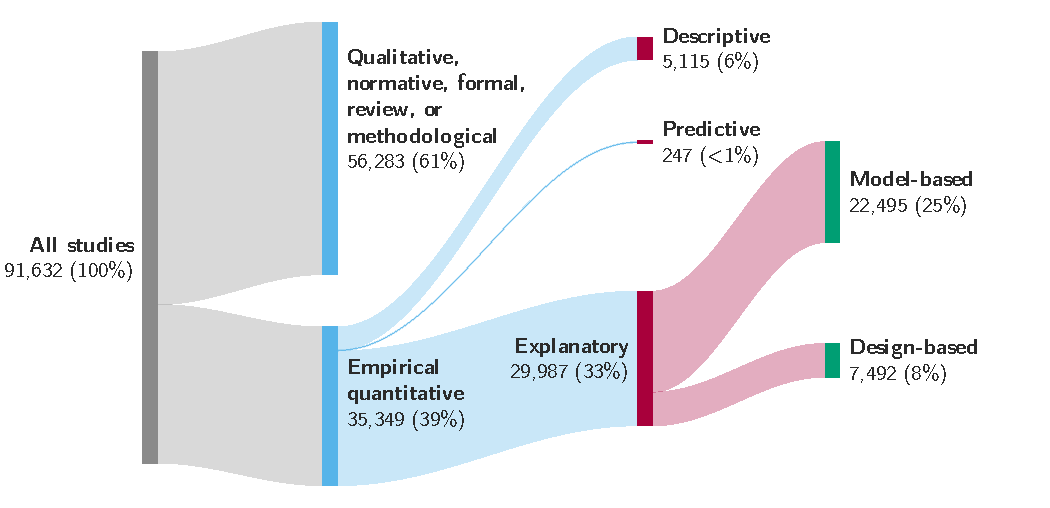
\includegraphics[height=0.62\textheight]{sankey_goals.pdf}

{\scriptsize \textbf{Model-based}: no clear research design; the causal claim relies on modeling assumptions. \textbf{Design-based}: a clear research design; the causal claim relies on how the cause was assigned.\par}
\slidesource{Torreblanca, Dinneen, Grossman \& Xu (2026), ``The Credibility Revolution in Political Science,'' arXiv:2601.11542, Figure 2: 91,632 articles in 156 political science journals, 2003--2023, classified with large language models. Percentages are shares of all 91,632 articles.}
\end{frame}  


\begin{frame}
  \frametitle{Description}
We ask questions to make a descriptive inference---that is, learn about some unobserved phenomenon on the basis of some set of observed facts\pause
\begin{itemize}
\item Are elections for the U.S. House of Representatives less competitive in the last several decades than
previously?
\item Do civil wars last longer in countries with rough terrain? \bigskip\pause
\end{itemize}
de Kadt \& Grzymala-Busse (2025), ``Good Description'' (SocArXiv, \href{https://doi.org/10.31235/osf.io/e74a9_v2}{\nolinkurl{doi:10.31235/osf.io/e74a9_v2}}):
\begin{itemize}
  \item Uncover facts in need of explanation, build theory, or help to evaluate and revise theory
  \item Clear, comparable, and complete
\end{itemize}
\end{frame}

\begin{frame}
  \frametitle{Prediction}
We ask questions about observations not in our data\pause
\begin{itemize}
\item Who will win the Democratic primary?
\item Which party will control the U.S. House after the \ifrelease next\else November 2026\fi{} midterm elections?
\end{itemize}
\end{frame}



\begin{frame}
  \frametitle{Explanation \& Causation}
We ask questions about counterfactuals.
\begin{itemize}
\item Would citizens have voted at a higher rate if a campaign worker had
contacted them in person?\pause
\item Would France have developed more quickly if it had developed
institutions of limited government in the late 17th and early 18th
century? \pause\bigskip
\end{itemize}
Questions of the form what would have happened to the behavior or outcomes
of people, cities or states if they had been subjected to some stimulus, $T$.
% 2026-10-12 (Yiqing): about people, never one person ("a particular individual"), since causal effects are not
% identified for an individual; the 450D line ends in \ldots (no 451, 452 or Bayesian statistics), as in the video.
\end{frame}

\begin{frame}
  \frametitle{This Course}
\textbf{Course Plan}\bigskip
\begin{itemize}\itemsep1em
\item Univariate Statistical Inference
\item What is Regression?
\item Simple Linear Regression
\item Multiple Linear Regression
\item Diagnosing and Fixing Problems
\item Extensions
\end{itemize}
\end{frame}


%\begin{frame}
%\frametitle{Regression and The Problem of Causal Inference}
%\bi
%\item Introduce potential outcomes model of causal inference with example. \pause
%\item Let us call $y_{i}^{T}$ the average income of citizens in
%a country if the country $i$ is a democracy, and $y_{i}^{C}$ the
%average income of citizens in the same country $i$ if the country is
%not a democracy.  \pause
%\item What we want to know substantively is the effect of
%democracy on income for country $i$.
%This is equal to the difference $\delta_{i}=y_{i}^{T}-y_{i}^{C}$. $\delta_{i}$ is the
%unit-level causal effect.\\
%\ei
%\end{frame}

%
%\begin{frame}
%\frametitle{Regression and The Problem of Causal Inference}
%
%\bi
%
%\item Notice in our example we have two well-defined causal states
%to which all members of the population of interest (countries) could
%be exposed. The two states are the $T$reatment (democracy) and
%$C$ontrol (not democracy). When a cause has many values, we refer to
%the alternative states as alternative treatments. \pause
%
%\item Given $\delta_{i}=y_{i}^{T}-y_{i}^{C}$, we can see a problem,
%we will never have a country $i$ both with and without democracy at
%the same time. The \textbf{\emph{fundamental problem of causal inference}} is
%that one can never observe the potential outcome under the treatment
%for those observed in the control state and one can never observe
%the potential outcome under the control state for those observed in
%the treatment state. One can never calculate unit-level causal
%effects. \ei
%\end{frame}
%
%\begin{frame}
%\frametitle{What can we do?}
%
%\noi We will never know the effect of having
%democracy on a country in particular but we may hope to learn the
%average effect that it will have on countries:   \pause
%
%\begin{eqnarray*}
%E[\delta] &=& E[Y^{T}-Y^{C}] \\
%&=& E[Y^{T}]-E[Y^{C}]
%\end{eqnarray*}
%
%\noi $E[\delta]$ is the \textbf{average treatment effect} or average causal effect. This equation is
%defined with reference to the population of interest, which in this
%case is all countries.
%\end{frame}
%
%\begin{frame}
%\frametitle{What can we do?}
%
%\noi \textbf{Average treatment effect on the treated (ATT).} In our example, this is
%expected what-if difference in income that would be observed if we
%could observe economic performance of a randomly selected democratic
%country under both democratic and non-democratic institutions.
%
%\begin{eqnarray*}
%E[\delta|D=T]&=&E[Y^{T}-Y^{C}|D=T] \\
%&=& E[Y^{T}|D=T]-E[Y^{C}|D=T]
%\end{eqnarray*}
%\end{frame}
%
%
%\begin{frame}
%\frametitle{Naive estimation}
%
%\noi So imagine we have access to data on lots of countries. Some
%countries have democracy and others do not. We may think of taking
%the average in both groups, and the difference between average
%incomes in countries with democracy and average incomes in countries
%without democracies. This is equal to:
%
%\begin{eqnarray*}
%\hat{\delta_{NAIVE}} &=& E[y_{i}|\text{democracy}]-E[y_{i}|\text{not democracy}] \\
%&=& E[y_{i}|d_{i}=T]-E[y_{i}|d_{i}=C]
%\end{eqnarray*}
%\end{frame}
%
%\begin{frame}
%\frametitle{Naive estimation}
%
%\noi In observational studies, the naive estimator rarely yields
%a consistent estimate of the average treatment effect because it
%converges to $E[Y|D=T]-E[Y|D=C]$ which is not equivalent to nor
%usually equal to the average causal effects defined above.
%\end{frame}
%
%\begin{frame}
%\frametitle{Naive estimation}
%
%\noi To see this: \\
%
%\bi
%\item Decompose the average treatment effect, letting $\pi$ equal to
%the proportion of the population that takes the treatment instead of
%the control.
%
%\begin{tiny}
%\begin{eqnarray*}
%E[\delta] &=& \{\pi E[Y^{T}|D=T]+(1-\pi)E[Y^{T}|D=C]\}-\{\pi
%E[Y^{C}|D=T]+(1-\pi)E[Y^{C}|D=C]\}
%\end{eqnarray*}
%\end{tiny}\pause
%\item So the average treatment effect is a function of five
%unknowns: the proportion of the population that is assigned to (or
%self-selects into) the treatment along with four additional
%expectations of the potential outcomes.
%\ei
%\end{frame}
%
%
%\begin{frame}
%\frametitle{Naive estimation}
%
%\bi
%\item Without additional assumptions, we can consistently estimate
%only three of the five unknowns: $\pi$, $E[Y^{T}|D=T]$,
%$E[Y^{C}|D=C]$ (by using the sample mean of the dummy treatment
%variable, sample mean of the observed outcome in the treatment
%group, and the sample mean of the observed outcome in the control
%group). \pause
%
%\item The remaining two unknowns $E[Y^{T}|D=C]$ and $E[Y^{C}|D=T]$
%are counterfactuals: the average outcome under the treatment for
%those in the control group and the average outcome under the control
%for those in the treatment group. Problem is we don't know what
%average income would have been of democratic countries if they had
%instead been non-democratic and we don't know what average income
%would have been of non-democratic countries if they had instead been
%democratic. \ei
%
%\end{frame}
%
%\begin{frame}
%\frametitle{Naive estimation}
%
%\noi \textbf{Expected Bias of the Naive Estimator}. From above,
%
%\begin{eqnarray*}
%\hat{\delta_{NAIVE}} &=& E[y_{i}|d_{i}=T]-E[y_{i}|d_{i}=C]
%\end{eqnarray*}
%
%\noi and this converges to $E[Y^{T}|D=T]-E[Y^{C}|D=C]$.
%
%\end{frame}
%
%
%\begin{frame}
%\frametitle{Naive estimation}
%
%\noi But rearranging our decomposition of the true average effect:
%
%\begin{eqnarray*}
%E[Y^{T}|D=T]-E[Y^{C}|D=C] &=& E[\delta] \\
%+ {E[Y^{C}|D=T]-E[Y^{C}|D=C]} \\
%+ (1-\pi){E[\delta|D=T]-E[\delta|D=C]}
%\end{eqnarray*}
%\pause
%\noi The first term is the true average treatment effect
%$E[\delta]$. The rest is bias and suggests two sources. The first is
%${E[Y^{C}|D=T]-E[Y^{C}|D=C]}$ is a \emph{baseline bias} equal to the
%difference in the average outcome in the absence of the treatment
%between those in the treatment group and those in the control group.
%The second is $(1-\pi){E[\delta|D=T]-E[\delta|D=C]}$ is a
%differential treatment effect bias equal to the expected difference
%in the treatment effect between those in the treatment and those in
%the control group.
%
%\end{frame}
%
%\begin{frame}
%\frametitle{Naive estimation}
%
%\noi \textbf{Expected Bias of the Naive Estimator--version 2}.
%
%\begin{eqnarray*}
%\hat{\delta_{NAIVE}} &=& E[y_{i}|d_{i}=T]-E[y_{i}|d_{i}=C]
%\end{eqnarray*}
%
%\noi and this converges to $E[Y^{T}|D=T]-E[Y^{C}|D=C]$.
%
%\end{frame}
%
%\begin{frame}
%\frametitle{Naive estimation}
%
%\noi Subtract and add $E[Y^{C}|D=T]$, we obtain
%
%\begin{tiny}
%\begin{eqnarray*}
%\hat{\delta_{NAIVE}} &=&
%E[Y^{T}|D=T]-E[Y^{C}|D=T]-E[Y^{C}|D=C]+E[Y^{C}|D=T] \\
%&=&E[Y^{T}-Y^{C}|D=T]+E[Y^{C}|D=T]-E[Y^{C}|D=C]
%\end{eqnarray*}
%\end{tiny}
%
%\bi
%\item The first term $E[Y^{T}-Y^{C}|D=T]$ is the conditional
%treatment effect referred to above---the effect of treatment on the
%treated: on average, in the treatment countries, what difference
%will democracy make? \pause
%
%\item The difference $E[Y^{C}|D=T]-E[Y^{C}|D=C]$ is the selection
%bias. It tells us that, beside the effect of democracy, there may be
%systematic differences between countries with democracy and other
%countries. Empirical methods try to solve this problem.
%\ei
%\end{frame}
%
%\begin{frame}
%\frametitle{Treatments we can control}
%\bi
%\item If we want to estimate the
%effect of a \textbf{treatment we can control}, we often design an
%\textbf{experiment} in which subjects are randomly assigned to alternative
%treatment and control groups. \pause
%
%\item In a randomized experiment, a sample of $N$ individuals/units
%is selected from the population. This sample is
%then divided randomly into two groups: the Treatment group ($N_{T}$
%individuals) and the Control group ($N_{C}$ individuals). Obviously
%$N_{T}+N_{C}=N$.\\
%\ei
%\end{frame}
%
%
%\begin{frame}
%\frametitle{Treatments we can control}
%
%\noi The Treatment group is then treated by stimulus $X$ (e.g.
%democracy) while the control group is not. Then the outcome $Y$ is
%observed and compared for both Treatment and Control groups. The
%effect of stimulus $X$ is measured in general by the difference in
%empirical means of $Y$ between Treatments and Controls: \pause
%
%\begin{eqnarray*}
%\hat{\delta} &=& \hat{E}(Y|T)-\hat{E}(Y|C)
%\end{eqnarray*} \pause
%
%\noi where $\hat{E}$ denotes the empirical mean. Since the Treatment
%has been randomly assigned, the difference
%$E[Y^{C}|T]-E[Y^{C}|C]$---selection bias---is equal to 0 (in the
%absence of the treatment the countries are the same).
%
%\end{frame}
%
%\begin{frame}
%\frametitle{Treatments we can control}
%
%\noi Therefore
%
%\begin{eqnarray*}
%E[Y|T]-E[Y|C] &=& E[Y^{T}-Y^{C}|T] \\
%\end{eqnarray*}
%
%\noi which is a causal parameter of interest. And will be equal to $E[Y^{T}-Y^{C}]$ if the treatment
%effect is the same across groups.\\
%
%\end{frame}
%
%
%\begin{frame}
%\frametitle{Treatments we do not control}
%
%\noi \textbf{Observational research} is
%an empirical investigation in which the investigator \textbf{does not
%control the assignment of treatments} to subjects. \pause
%
%\bi
%\item This means randomization designs are infeasible and there is usually no
%reason to think $E[Y^{C}|T]-E[Y^{C}|C]=0$ making naive estimation unconvincing\pause
%\item The observational researcher has observed data: $Y$, the
%outcome variable, $D$, the treatment status variable, and wants to
%determine the causal effect of $D$ on $Y$. \pause
%\item This is the challenge of lots of scholarship in the social
%sciences---to determine how best to learn from the data the world
%generates. \ei
%\end{frame}
%
%
%\begin{frame}
%\frametitle{Conditioning Strategies--Regression}
%
%\noi Naive estimation with regression:
%
%\begin{eqnarray*}
%Y&=& \alpha + \delta_{NAIVE}D + \epsilon
%\end{eqnarray*}
%
%\noi To interpret this as a causal effect, need to assume
%$D$ and $\epsilon$ are uncorrelated. Roughly, the same things
%that would make this not true are the things that in the potential
%outcomes framework make $E[Y^{C}|T]-E[Y^{C}|C]\neq0$
%\end{frame}
%
%\begin{frame}
%\frametitle{Conditioning Strategies--Regression}
%
%\noi Regression adjustment for otherwise omitted variables:
%
%\begin{eqnarray*}
%Y&=& \alpha + \delta D + X \beta + \epsilon
%\end{eqnarray*}
%
%\noi Roughly by now ``controlling for $X$'', $\delta$ can be interpreted as a causal estimate
%if willing to assume that:
%\bi
%\item $D$ is uncorrelated with $\epsilon$ for each subset of observations
%identified by the values of $X$
%\item the causal effect does not vary with $X$
%\item the relationship between $X$ and
%$Y$ is linear or a fully flexible parameterization of $X$ is used.
%\ei
%
%\noi Essentially, in the potential outcomes framework,
%we can make the weaker assumption that $E[Y^{C}|T,X]-E[Y^{C}|C,X]=0$ (\textbf{It is still a really strong assumption.})
%\end{frame}
%

%\begin{frame}
%\frametitle{What is regression for?}
%
%\bigskip
%\bi
%\item Answering descriptive questions
%\item Answering predictive questions
%\item Answering causal question---at least a starting point for doing so
%\ei
%\bigskip
%
%\end{frame}


\end{document}
